\documentclass{article}[letterpaper]
\usepackage[top=.75in,left=.8in,right=1in,bottom=1in]{geometry}
\usepackage{algorithm} 
\usepackage{algpseudocode} 
\usepackage{graphicx}
\usepackage{fancyhdr}

\setlength\parindent{0pt}
\setlength{\parskip}{1em}
\pagestyle{fancy}
\fancyhf{}
\lfoot{CS 444 AI Notes -- Search Problems and Uninformed Search}
\rfoot{Page \thepage}


\begin{document}

{\huge CS 444 Notes -- Search Problems and Uninformed Search \footnote{These notes are heavily based on work by Nikhil Sharma and
others Berkley instructors}}



\section*{Learning Objectives/Outcomes}
The learning outcomes/objectives are:
\begin{itemize}
\item define a problem given its 5 components (section 3.1.1 in the textbook)
\item define a world state and given a problem, define the minimum required world state representation
\item Define the difference between a state space graph and a search tree.  Given a problem, be able to draw a
state space graph and/or define the size of the state space.
\item Define completeness, optimality, branching factor, solution depth, goal state, and successor function with respect to search problems
\item Characterize the DFS, BFS, UCS, DLS, and IDS algorithms using these properties: completeness, optimality, running time, and space
complexity.  Be able to trace the execution of each of these algorithms given a problem.
\end{itemize}


\section*{State Space and Search Problems}
In order to create a rational planning agent, we need a way to mathematically express the given environment in which the agent will exist. To do this, we must formally express a \textbf{search problem} -given our agent’s current \textbf{state} (its configuration within its environment), how can we arrive at a new state that satisfies its goals in the best possible way? Formulating such a problem requires four things: 
\begin{itemize}
\item A \textbf{state space} -The set of all possible states that are possible in your given world 
\item A \textbf{successor function} - A function that takes in a state and an action and computes the cost of performing that action as well as the successor state, the state the world would be in if the given agent performed that action
\item A \textbf{start state} -The state in which an agent exists initially
\item A \textbf{goal test} -A function that takes a state as input, and determines whether it is a goal state

\end{itemize}

Fundamentally, a search problem is solved by first considering the start state, then exploring the state space using the successor function, iteratively computing successors of various states until we arrive at a goal state, at which point we will have determined a path from the start state to the goal state (typically called a \textbf{plan}). The order in which states are considered is determined using a predetermined \textbf{strategy}. We’ll cover types of strategies and their usefulness shortly. 

Before we continue with how to solve search problems, it’s important to note the difference between a \textbf{world state}, and a \textbf{search state}. A world state contains all information about a given state, whereas a search state contains only the information about the world that’s necessary for planning (primarily for space effiency reasons). To illustrate these concepts, we’ll introduce the hallmark motivating example of this course Pacman. The game of Pacman is simple: Pacman must navigate a maze and eat all the (small) food pellets in the maze without being eaten by the malicious patrolling ghosts. If Pacman eats one of the (large) power pellets, he becomes ghost-immune for a set period of time and gains the ability to eat ghosts for points.

%% pacman fig here

Let’s consider a variation of the game in which the maze contains only Pacman and food pellets. We can pose two distinct search problems in this scenario: pathing and eat-all-dots. Pathing attempts to solve the problem of getting from position ($x_1,y_1$) to position ($x_2,y_2$) in the maze optimally, while eat all dots attempts to solve the problem of consuming all food pellets in the maze in the shortest time possible. Below, the states, actions, successor function, and goal test for both problems are listed:

\begin{minipage}{0.5\textwidth}
\begin{itemize}
\item \textbf{Pathing}
\begin{itemize}
\item States (x,y) locations
\item Actions: North, South, East, West
\item Successor: Update location only
\item Goal test: Is (x,y) = END?
\end{itemize}
\end{itemize}
\end{minipage}
\begin{minipage}{0.5\textwidth}
\begin{itemize}
\item \textbf{Eat-all-dots} 
\begin{itemize}
\item States: (x, y) location, dot booleans
\item Actions: North, South, East, West
\item Sucessor: Update location and booleans
\item Goal Test: Are all dot booleans false?
\end{itemize}
\end{itemize}
\end{minipage}

Note that for pathing, states contain less information than states for eat-all-dots, because for eat-all-dots we must maintain an array of booleans corresponding to each food pellet and whether or not it’s been eaten in the given state. A world state may contain more information still, potentially encoding information about things like total distance traveled by Pacman or all positions visited by Pacman on top of its current (x,y) location and dot booleans.


\section*{State Space Size}
An important question that often comes up while estimating the computational runtime of solving a search problem is the size of the state space. This is done almost exclusively with the \textbf{fundamental counting principle}, which states that if there are n variable objects in a given world which can take on 
$x_1, x_2, ..., x_n$ different values respectively, then the total number of states is $x_1\cdot x_2 \cdot ... \cdot x_n$. Let’s use Pacman to show this concept by example:

Let’s say that the variable objects and their corresponding number of possibilities are as follows:
\begin{itemize}
\item  Pacman positions -Pacman can be in 120 distinct ($x,y$) positions, and there is only one Pacman
\item Pacman Direction -this can be North, South, East, or West, for a total of 4 possibilities 
\item Ghost positions -There are two ghosts, each of which can be in 12 distinct ($x,y$) positions
\item Food pellet configurations -There are 30 food pellets, each of which can be eaten or not eaten
\end{itemize}

Using the fundamental counting principle, we have 120 positions for Pacman, 4 directions Pacman can be facing, $12 \cdot 12$ ghost configurations (12 for each ghost), and $2 \cdot 2 \cdot ...\cdot 2 = 2^{30}$ food pellet configurations (each of 30 food pellets has two possible values - eaten or not eaten). This gives us a total state space size of $120 \cdot 4 \cdot 12^2 \cdot 2^{30}$.

\section*{State Space Graphs and Search Trees}
Now that we’ve established the idea of a state space and the four components necessary to completely define one, we’re almost ready to begin solving search problems. The final piece of the puzzle is that of state space graphs and search trees.

Recall that a graph is defined by a set of nodes and a set of edges connecting various pairs of nodes. These edges may also have weights associated with them. A \textbf{state space graph} is constructed with states representing nodes, with directed edges existing from a state to its successors. These edges represent actions, and any associated weights represent the cost of performing the corresponding action. Typically, state space graphs are much too large to store in memory (even our simple Pacman example from above has $\approx 10^{13}$ possible states, yikes!), but they’re good to keep in mind conceptually while solving problems. It’s also important to note that in a state space graph, each state is represented exactly once, there’s simply no need to represent a state multiple times, and knowing this helps quite a bit when trying to reason about search problems.

Unlike state space graphs, our next structure of interest, \textbf{search trees}, have no such restriction on the number of times a state can appear. This is because though search trees are also a class of graph with states as nodes and actions as edges between states, each state/node encodes not just the state itself, but the entire path (or plan) from the start state to the given state in the state space graph. Observe the state space graph and corresponding search tree below:

\begin{figure}
\begin{tabular}{c c}
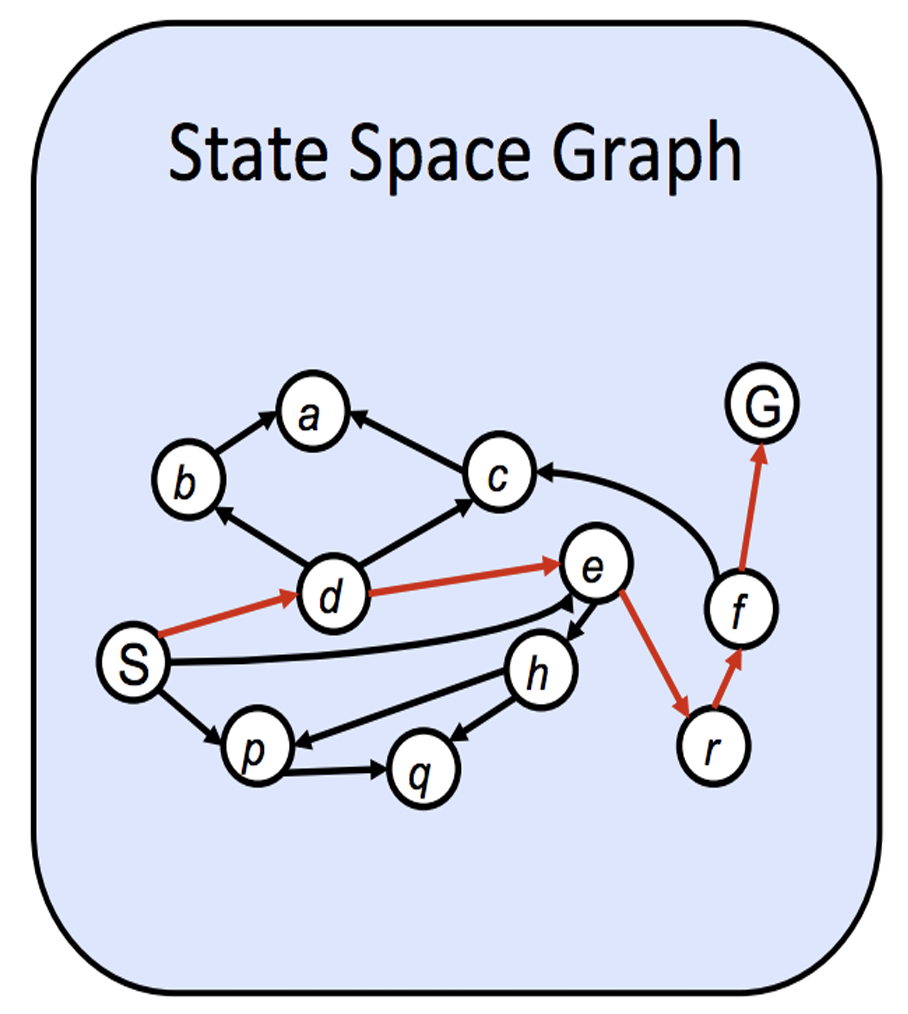
\includegraphics[width=0.44\textwidth]{figs/StateSpaceGraph} & 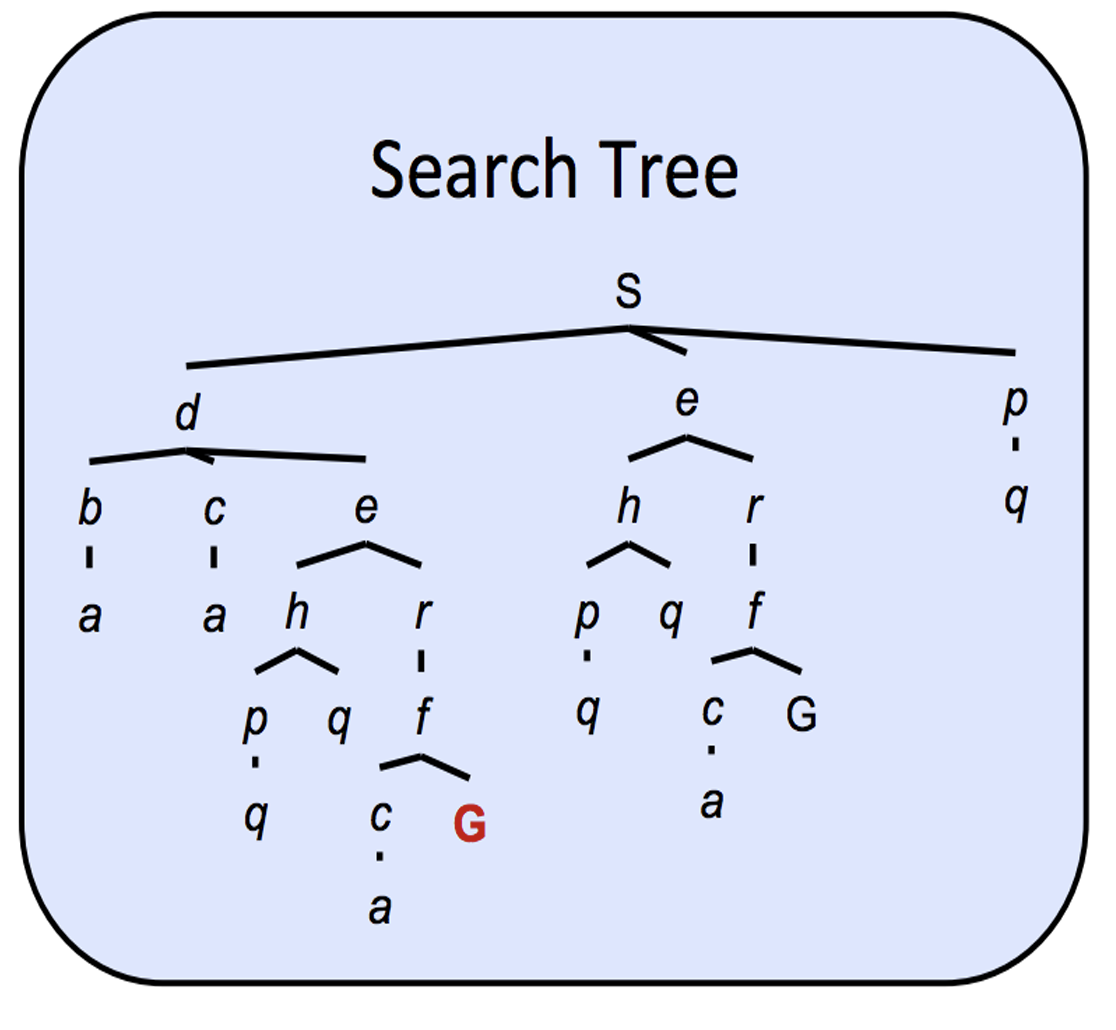
\includegraphics[width=0.52\textwidth]{figs/SearchTree}  \\
\end{tabular}
\caption{Each node in the search tree is an entire \textbf{PATH} in the state space graph.  We construct both \textbf{on demand} - and 
we construct as little as possible.  }
\end{figure}


The highlighted path $(S \rightarrow d \rightarrow e \rightarrow r \rightarrow f \rightarrow G$) in the given state space graph is represented in the corresponding search tree by following the path in the tree from the start state S to the highlighted goal state G. Similarly, each and every path from the start node to any other node is represented in the search tree by a path from the root S to some descendant of the root corresponding to the other node. Since there often exist multiple ways to get from one state to another, states tend to show up multiple times in search trees. As a result, search trees are greater than or equal to their corresponding state space graph in size.

\section*{Uninformed Search}
The standard protocol for finding a plan to get from the start state to a goal state is to maintain an outer
\textbf{fringe} of partial plans derived from the search tree. We continually \textbf{expand} our fringe by removing a node
(which is selected using our given \textbf{strategy}) corresponding to a partial plan from the fringe, and replacing
it on the fringe with all its children. Removing and replacing an element on the fringe with its children
corresponds to discarding a single length $n$ plan and bringing all length ($n+1$) plans that stem from it into
consideration. We continue this until eventually removing a goal state off the fringe, at which point we
conclude the partial plan corresponding to the removed goal state is in fact a path to get from the start state
to the goal state. Practically, most implementations of such algorithms will encode information about the
parent node, distance to node, and the state inside the node object. This procedure we have just outlined is
known as \textbf{tree search}, and the pseudocode for it is presented below:

\begin{algorithm}
	\caption{Tree-Search}
	\begin{algorithmic}[1]
   	        \Function{Tree-Search}{problem}~returns a solution or failure
	           \State fringe $\leftarrow$ INSERT(MAKE-NODE(INITIAL-STATE[problem]), fringe)
	           \Loop
	               \If {fringe is empty} 
	                   return failure
	               \EndIf
	            \State node $\leftarrow$ REMOVE-FRONT(fringe)
	            \If {GOAL-TEST(problem, STATE[node])}
	                return node
	            \EndIf
	            \For {child-node in EXPAND(STATE[node], problem)}
	               \State fringe $\leftarrow$ INSERT(child-node, fringe)
	            \EndFor
	         \EndLoop
	         \EndFunction
	\end{algorithmic} 
\end{algorithm} 

When we have no knowledge of the location of goal states in our search tree, we are forced to select our
strategy for tree search from one of the techniques that falls under the umbrella of uninformed search.
We’ll now cover three such strategies in succession: \textbf{depth-first search}, \textbf{breadth-first search}, and \textbf{uniform
cost search}. Along with each strategy, some rudimentary properties of the strategy are presented as well, in
terms of the following:

\begin{itemize}
\item The \textbf{completeness} of each search strategy - if there exists a solution to the search problem, is the
strategy guaranteed to find it given infinite computational resources?

\item The \textbf{optimality} of each search strategy - is the strategy guaranteed to find the lowest cost path to a
goal state?

\item The \textbf{branching factor} $b$ - The increase in the number of nodes on the fringe each time a fringe node
is dequeued and replaced with its children is $\mathcal{O}(b)$. At depth k in the search tree, there exists 
$\mathcal{O}(b^k)$ nodes.

\item The maximum depth $m$.

\item The depth of the shallowest solution $s$ (sometimes referred to as $d$ as well).  

\end{itemize}

\section*{Depth-First Search}
\begin{itemize}
\item \textit{Description} - Depth-first search (DFS) is a strategy for exploration that always selects the deepest
fringe node from the start node for expansion.

\item \textit{Fringe representation} - Removing the deepest node and replacing it on the fringe with its children
necessarily means the children are now the new deepest nodes - their depth is one greater than the
depth of the previous deepest node. This implies that to implement DFS, we require a structure that
always gives the most recently added objects highest priority. A last-in, first-out (LIFO) stack does
exactly this, and is what is traditionally used to represent the fringe when implementing DFS.

\begin{figure}
\centering
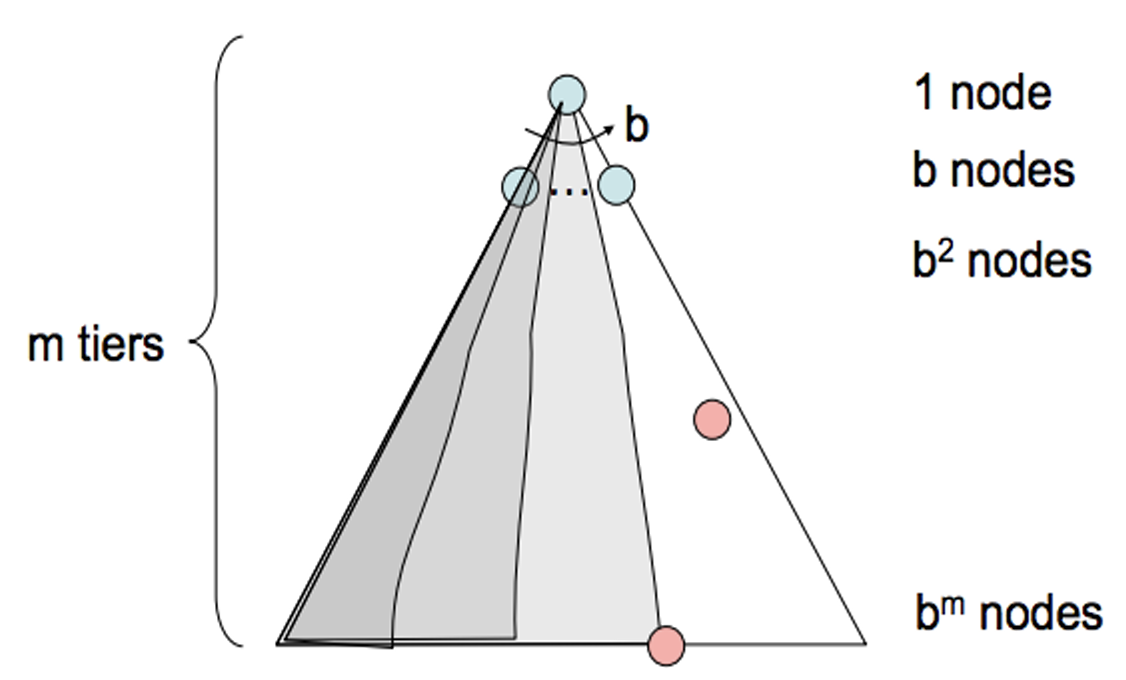
\includegraphics[width=0.44\textwidth]{figs/DFS} 
\end{figure}

\item \textit{Completeness} - Depth-first search is not complete. If there exist cycles in the state space graph, this
inevitably means that the corresponding search tree will be infinite in depth. Hence, there exists the
possibility that DFS will faithfully yet tragically get "stuck" searching for the deepest node in an
infinite-sized search tree, doomed to never find a solution.

\item \textit{Optimality} - Depth-first search simply finds the "leftmost" solution in the search tree without regard
for path costs, and so is not optimal.

\item \textit{Time Complexity} - In the worst case, depth first search may end up exploring the entire search tree.
Hence, given a tree with maximum depth m, the runtime of DFS is $\mathcal{O}(b^m)$.

\item \textit{Space Complexity} - In the worst case, DFS maintains $b$ nodes at each of $m$ depth levels on the fringe.
This is a simple consequence of the fact that once $b$ children of some parent are enqueued, the nature
of DFS allows only one of the subtrees of any of these children to be explored at any given point in
time. Hence, the space complexity of BFS is $\mathcal{O}(bm)$.
\end{itemize}

\section*{Breadth-First Search}
\begin{itemize}
\item \textit{Description} - Breadth-first search is a strategy for exploration that always selects the \textit{shallowest}
 fringe node from the start node for expansion.


\item \textit{Fringe representation} - If we want to visit shallower nodes before deeper nodes, we must visit nodes in their order of insertion. Hence, we desire a structure that outputs the oldest enqueued object to represent our fringe. For this, BFS uses a first-in, first-out (FIFO) queue, which does exactly this.

\begin{figure}
\centering
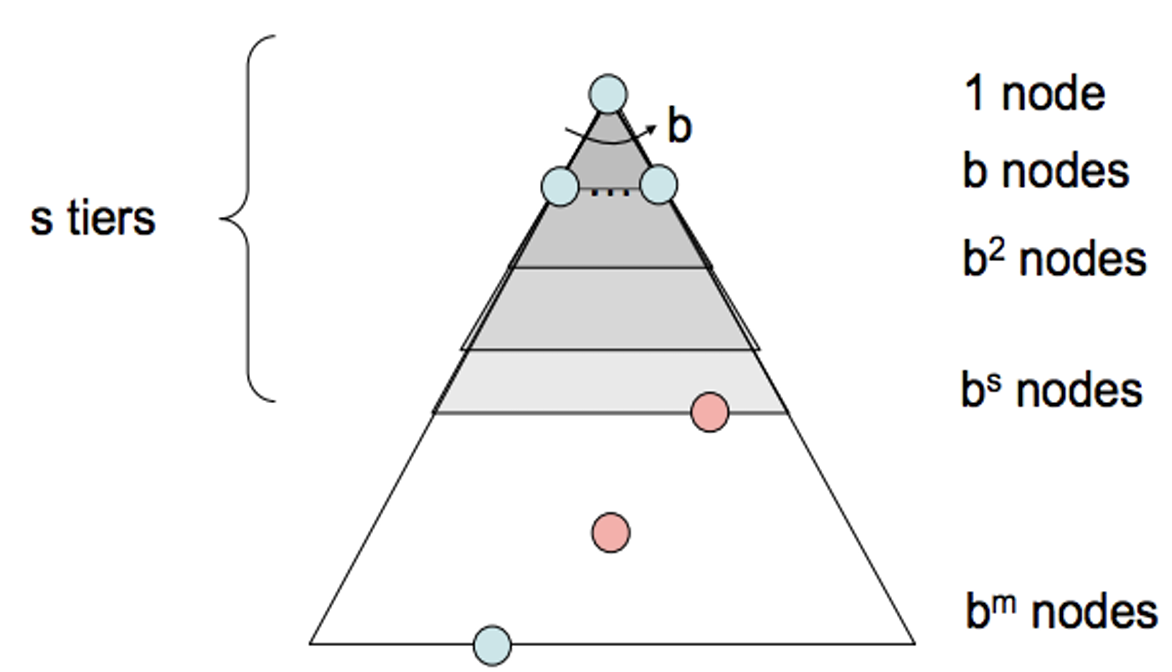
\includegraphics[width=0.44\textwidth]{figs/BFS} 
\end{figure}

\item \textit{Completeness} - If a solution exists, then the depth of the shallowest node $s$ must be finite, so BFS must eventually search this depth. Hence, it’s complete.

\item \textit{Optimality} -  BFS is generally not optimal because it simply does not take costs into consideration when determining which node to replace on the fringe. The special case where BFS is guaranteed to be optimal is if all edge costs are equivalent, because this reduces BFS to a special case of uniform cost search, which is discussed below.

\item \textit{Time Complexity} - We must search $1+b+b^2+...+b^s$ nodes in the worst case, since we go through all nodes at every depth from 1 to $s$. Hence, the time complexity is $\mathcal{O}(bs)$.

\item \textit{Space Complexity} -The fringe, in the worst case, contains all the nodes in the level corresponding to the shallowest solution. Since the shallowest solution is located at depth $s$, there are $\mathcal{O}(b^s)$ nodes at this depth.
\end{itemize}

\section*{Depth Limited Search -- DLS}
\begin{itemize}
\item \textit{Description} - Perform a DFS but impose a limit $\ell$ that defines the maximum depth to explore.  You
can think of DFS is just DLS with $\ell = \infty$.

\item \textit{Fringe representation} - Just like DFS, we require a structure that
always gives the most recently added objects highest priority, so a LIFO stack is used.  Once a depth of $\ell$ 
is reached, the node is treated as a leaf (it has no successor states).

\item \textit{Completeness} - The max depth of the tree to be searched is $\ell$.  If $\ell < m$ (where $m$ is the depth
of the shallowest solution), DLS is incomplete.  

\item \textit{Optimality} -  DLS is not guaranteed to be optimal in the cases where $\ell > m$.  

\item \textit{Time Complexity} - We must search $1+b+b^2+...+b^s$ nodes in the worst case, since we go through all nodes at every depth from 1 to $\ell$. Hence, the time complexity is $\mathcal{O}(b^{\ell})$.

\item \textit{Space Complexity} -In the worst case, DLS maintains $b$ nodes at each of $l$ depth levels on the fringe.
This is a simple consequence of the fact that once $b$ children of some parent are enqueued, the nature
of DLS allows only one of the subtrees of any of these children to be explored at any given point in
time. Hence, the space complexity of DLS is $\mathcal{O}(bm)$.


\end{itemize}

\section*{Iterative Deepening search(IDS)}
\begin{itemize}
\item \textit{Description} - Perform a DLS, and keep increasing the depth limit $\ell$ by one until a solution is found.  This
may seem wasteful, but, given that most of the nodes are at the bottom level of the tree, and that the next to bottom level is only 
generated twice (and the top of the tree does not contain that many nodes), it works quite well in practice.  

\item \textit{Fringe representation} - Same as DLS.

\item \textit{Completeness} -  IDS is complete (given a finite $b$).  If a goal state exists, it must have some finite path, and therefore will be found.
IDS addresses the infinite-path problem by always enforcing a max depth limit via DLS.  

\item \textit{Optimality} -  IDS is optimal IF the costs of each edge are the same.

\item \textit{Time Complexity} - For a solution a depth $d$, those nodes are generated once (and there are $b^d$ of these nodes).
The nodes at the prior level are generated $(2) * b^{d-1}$, and working our way back to the root node, which is generated $d$ times.
We get the series:
\begin*{equation}
$N(IDS) = d(b) + (d-1)b^2 + (d-2)b^3 + ... + 2b^{d-1} + b^{d}$
\end*{equation}
Which gives the same big-Oh complexity, $\mathcal{O}^{d}$ (the same as BFS).

\item \textit{Space Complexity} -Same as DLS, maintains at most $\mathcal{O}(bd)$ nodes  (where $d$ is the shallowest depth of
a solution).
\end{itemize}



\section*{Uniform First Search}
\begin{itemize}
\item \textit{Description} - Uniform cost search (UCS) is a strategy for exploration that always selects the
\textit{lowest cost} fringe node from the start node for expansion.

\item \textit{Fringe representation} -
To represent the fringe for UCS, the choice is usually a heap-based priority queue, where the weight for a given enqueued node $v$ is the path cost from the start node to $v$, or the \textit{backward cost} of $v$. Intuitively, a priority queue constructed in this manner simply reshuffles itself to maintain the desired ordering by path cost as we remove the current minimum cost path and replace it with its children.

\item \textit{Completeness} - Uniform cost search is complete. If a goal state exists, it must have some finite length shortest path; hence, UCS must eventually find this shortest length path.

\begin{figure}[h]
\centering
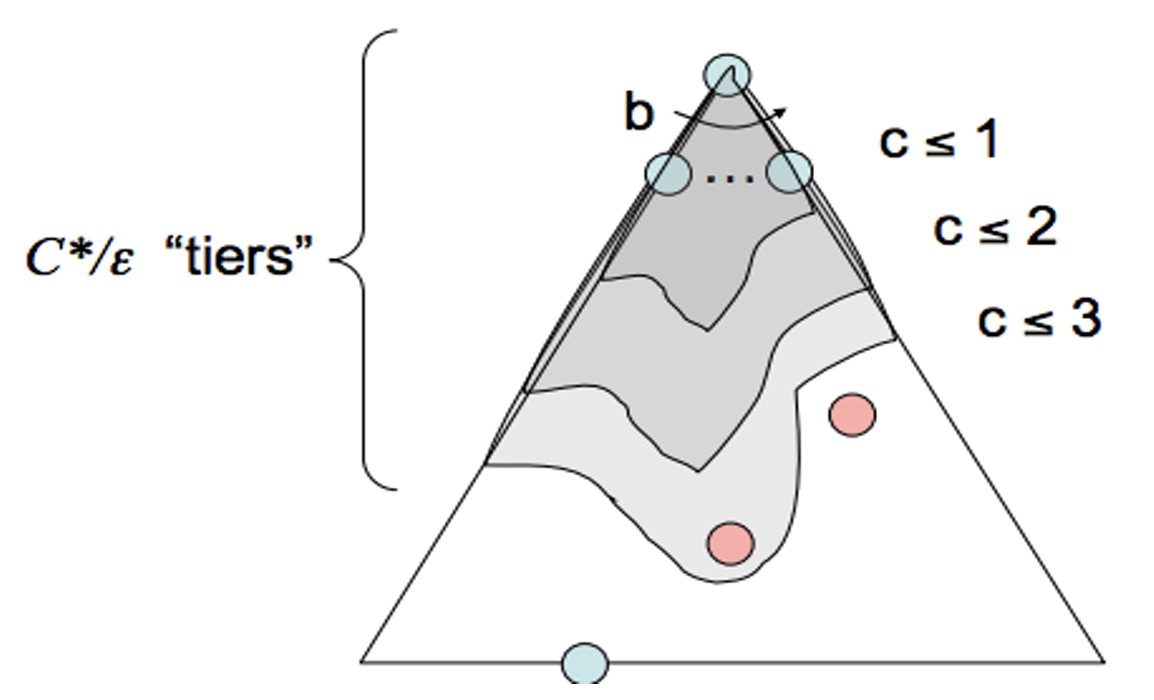
\includegraphics[width=0.44\textwidth]{figs/UCS} 
\end{figure}


\item \textit{Optimality} - UCS is also optimal if we assume all edge costs are nonnegative. 
By construction, since we explore nodes in order of increasing path cost, we’re guaranteed to find the lowest-cost path to a goal state. The strategy employed in Uniform Cost Search is identical to that of \textbf{Dijkstra’s algorithm}, 
and the chief difference is that UCS terminates upon finding a solution state instead of finding the shortest path to all states. 
Note that having negative edge costs in our graph can make nodes on a path have decreasing length, ruining our guarantee of optimality. (See Bellman-Ford algorithm for a slower algorithm that handles this possibility)


\item \textit{Time Complexity} - 
Let us define the optimal path cost as $C^*$ and the minimal cost between two nodes in the state space graph as $\epsilon$. 
Then, we must roughly explore all nodes at depths ranging from 1 to $C^*/\epsilon$, leading to a runtime of $\mathcal{O}(b^{C^*/\epsilon})$.

\item \textit{Space Complexity}  - -Roughly, the fringe will contain all nodes at the level of the cheapest solution, so the space complexity of UCS is estimated as $\mathcal{O}(b^{C^*/\epsilon})$.
\end{itemize}

\newpage

\section*{Summary on Uninformed Search}
As a parting note about uninformed search, it’s critical to note that the three strategies outlined above are fundamentally the same - differing only in expansion strategy, with their similarities being captured by the tree search pseudocode presented above.
\begin{figure}[h!]
\begin{tabular}{l | c | c | c | c | c | c}
Criterion & Breadth-First & Uniform-Cost & Depth-First & Depth-Limited & Iterative Deepening & Bidirectional  \\ \hline \hline
Complete? & Yes\textsuperscript{A} & Yes \textsuperscript{A}  & No & No & Yes \textsuperscript{A} & Yes \textsuperscript{A,D} \\ \hline
Time           & $\mathcal{O}(b^d)$       &  $\mathcal{O}(b^{1 + \lfloor C^*/ \epsilon \rfloor)}$ & $\mathcal{O}(b^m) $ & $\mathcal{O}(b^\ell) $ & $\mathcal{O}(b^d)$  & $\mathcal{O}(b^{d/2})$ \\ \hline  
Space         & $\mathcal{O}(b^d)$       &  $\mathcal{O}(b^{1 + \lfloor C^*/ \epsilon \rfloor)}$  & $\mathcal{O}(bm)$ &   $\mathcal{O}(b\ell) $  & $\mathcal{O}(bd)$  & $\mathcal{O}(b^{d/2})$ \\ \hline  
Optimal       &  Yes\textsuperscript{C} & Yes                                                                             & No                          & No                               & Yes\textsuperscript{C} & Yes\textsuperscript{C,D} \\ \hline
\end{tabular}
\caption{Figure from Russell/Norvig.  $b$ is the branching factor; $d$ is the depth of the shallowest solution; $m$ is the maximum depth of the search tree; $\ell$ is
the depth limit.  Footnote explanations: \textsuperscript{A} - complete if $b$ is finite;
\textsuperscript{B} - complete if step costs $\ge \epsilon$ for positive $\epsilon$;
\textsuperscript{C} - optimal if step costs are all identical;
\textsuperscript{D} - if both directions use breadth-first search
}
\end{figure}
\end{document}